\subsection{Elección de herramientas en la arquitectura de aplicación de IPFS}

\paragraph{Manejo de conexión}
%todo: redactar
OrbitDB no se responsabiliza de manejar las conexiones, tampoco le importa, ya que te asegura que eventualmente la base de datos va a estar sincronizada entre peers, aunque se caigan las conexiones o te conectes mas tarde, todo se va a sincronizar sin conflictos eventualmente. Por lo tanto delega esa responsabilidad a \textbf{Helia} \cite{helia} la cual es la implementación de IPFS en los lenguajes javascript/typescript, que a su vez delega la responsabilidad a \textbf{LibP2P} \cite{libp2p} y de la cual tenemos que hacer uso nosotros para manejar las conexiones.

LibP2P es una colección de protocolos y utilidades para facilitar la implementación de una red peer-to-peer. Al crear un nodo de LibP2P se tiene que elegir como conformarlo en base a un conjunto modular de herramientas, dentro de los que se encuentran mecanismos de seguridad, de transporte, descubrimiento de pares, entre otros. Cada una de estas herramientas es importante y hace que el nodo funcione como queramos, más adelante explicaremos la decisión para cada herramienta elegida, sin embargo ahora nos vamos a centrar en dos protocolos de interés necesarios para solucionar el problema de manejo de conexión. Los protocolos de transporte y de descubrimiento de peers.

Los protocolos de transporte son los encargados de la comunicación entre nodos, de manera similar a la capa de transporte presente en toda red convencional. Se basan en tipos de transporte ya existentes, adaptados al uso peer-to-peer. Como lo son TCP, QUIC o WebSockets. Sin embargo no todos los transportes nos son útiles y la decisión de cual protocolo utilizar no es sencilla.

Uno de los requisitos de esta infraestructura era la posibilidad de utilizarla para crear aplicaciones que se puedan utilizar desde un entorno web, como es el caso de un usuario queriendo acceder a la wiki desde un navegador. Lo que sucede es que el entorno web no es muy amigable con las conexiones. Los navegadores están construidos sobre HTTP(S), un protocolo sin estado basado en solicitudes y respuestas. El cliente (navegador) envía una solicitud y luego espera una respuesta. Las conexiones se manejan en la capa de transporte y no mediante HTTP(S). Los navegadores imponen reglas estrictas, como los requisitos de certificados y el bloqueo de políticas de origen cruzado (cross-origin).

Es por esto que por razones de seguridad, no es posible que un navegador establezca una conexión TCP o QUIC sin procesar directamente desde el navegador, ya que todas las conexiones deben cumplir con los requisitos de Contexto Seguro (Secure Context), como por ejemplo que los mensajes se entreguen a través de TLS.

Es por esta razón que la infraestructura debe hacer una diferenciación entre nodos que se ejecuten desde un entorno independiente, como es el caso de \textbf{node.js} \cite{nodejs} y nodos que se ejecuten en un entorno web, únicamente para asignarle los protocolos de transporte correspondientes a su entorno.

Hay 2 conexiones que se tienen que resolver, la conexión entre nodos independientes y la conexión desde un nodo web a un nodo independiente.

Para los nodos independientes la solución es sencilla y el protocolo utilizado es TCP, con el cual pueden comunicarse entre sí y con otros nodos independientes de la red. El problema viene que, como explicamos, TCP no nos sirve para comunicar desde un nodo web a un nodo independiente, por lo tanto hay que explorar alternativas.

Al momento de comenzar con el desarrollo del repositorio de conocimiento, la implementación de LibP2P en javascript ofrecía dos formas para resolver la conexión de web a nodo independiente.

La primera alternativa analizada y más conocida es la de utlizar \textbf{WebSockets} \cite{websocket}. El protocolo WebSocket permite “secuestrar” una conexión HTTP y tras una solicitud para asegurar la conexión, el navegador obtiene acceso directo a la conexión TCP subyacente, permitiendo comunicación bidireccional persistente. Sin embargo esta alternativa no nos de fue de utilidad ya que para lograr esta mejora de conexión es necesario contar con un dominio o certificado por una autoridad certificadora, cosa que muy probablemente los nodos y usuarios utilizando la infraestructura no tengan.

La otra alternativa adicional considerada fue el uso de la técnica conocida como \textbf{Hole Punching} \cite{hole-punching}, una técnica muy interesante que permite que nodos privados —es decir, aquellos ubicados detrás de un firewall o en redes donde no pueden recibir conexiones entrantes, como hogares, redes corporativas o dispositivos móviles— puedan establecer conexiones con otros nodos. Para lograrlo, un nodo público actúa como intermediario, escuchando por ellos, este nodo es denominado como \textbf{Relay}. Esto nos sirve ya que un nodo web actua como un nodo privado ya que, aunque no pueden aceptar conexiones entrantes, sí pueden iniciarlas; así, todo el tráfico pasa a través del nodo intermediario, permitiendo una comunicación efectiva. No obstante, esta opción presenta una limitación relevante: el soporte para esta funcionalidad aún se encuentra en desarrollo en la implementación de libp2p para JavaScript, y no fue posible obtener un funcionamiento estable en el contexto de nuestro proyecto.

Al ver que ambas formas provistas no nos eran de utilidad nos puso en un lugar difícil, dado que de no poder lograr la conexión significaría que esta infraestructura no iba a poder funcionar, sin embargo el desarrollo e investigación continuó aunque no sabíamos si se iba a poder lograr una forma exitosa, lo cual era un riesgo. Sin embargo en al rededor de la mitad del proyecto, el soporte para una nueva alternativa se implementó.

Esta nueva alternativa es la conocida como \textbf{AutoTLS} \cite{autotls} la cual conciste en obtener un certificado y dominio dependiente del ID del nodo usando el protocolo conocido como \textbf{ACME} \cite{acme}, del cual libp2p provee un servicio DNS de bien público que responderá en nombre de cualquier usuario de Internet. De esta manera se puede usar el método de websockets de manera segura gracias al certificado que se obtiene. El funcionamiento de esta alternativa nos permitió continuar con el desarrollo y poder probar la infraestructura que se estaba creando. Sin embargo esta alternativa seguía teniendo algunas desventajas, la primera era que su conexión era muy inestable, al también ser una nueva alternativa experimental sufría de problemas. Pero más importante aún era que iba en contra de la filosofía que intentábamos lograr, que es la de una descentralización, como se requiere de un servidor de terceros para obtener el certificado, se depende de la disponibilidad de este servidor, y de no estar significaría que los nodos no puedan conectarse, por lo tanto aún necesitábamos una mejor alternativa.

Un tiempo después surge el soporte de una nueva alternativa, la cual ya teniamos conocimiento porque existía en otras implementaciones de libp2p en otros lenguajes y estaba en desarrollo para la implementación en javascript. Esta alternativa es la conocida como \textbf{WebRTC} \cite{webrtc} mas especificamente su implementación directa para conectar desde web a nodo independiente llamada \textbf{WebRTC-Direct}.  Curiosamente hasta los mismos desarrolladores de libp2p recomendaban utilizar otras implementaciones en otros lenguajes para resolver la conexión web a nodo independiente hasta que el soporte de esta alternativa o otra muy similar se completen, citando: "Therefore, until WebRTC-Direct or WebTransport support is added to js-libp2p in Node.js, it’s much easier to use go-libp2p." \cite{differences-nodejs-browser} Lo cual no podiamos permitirnos por el requisito de permitir utilizarlo en aplicaciones web y que orbitdb tambien se encuentra en el ecosistema de javascript.

WebRTC es un conjunto de estándares abiertos y APIs web que permiten a las aplicaciones web establecer conectividad directa para conferencias de audio y video, así como para intercambiar datos arbitrarios. LibP2P lo utiliza para lograr una conexión directa y sin necesidad de usar un certificado TLS. De esta manera logramos que ya no sea necesario utilizar AutoTLS y podemos conectarnos corrementamente desde un nodo web a un nodo independiente usando WebRTC-Direct.

De esta manera la topología de conexiones resultante entre nodos independientes y nodos web resulta de la siguiente forma: 

\begin{figure}[H]
    \centering
    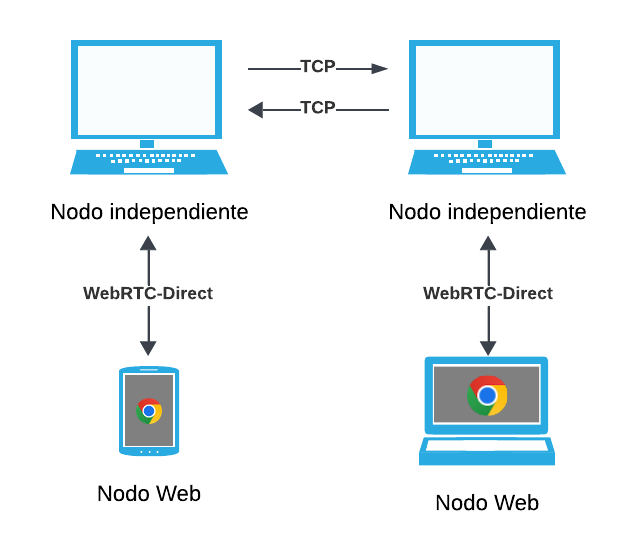
\includegraphics[width=0.5\linewidth]{img/solucion-ipfs/topologia.png}
    \caption{Topología de conexiones entre nodos independientes y nodos web.}
    \label{fig:bdd-articulos}
\end{figure}